\documentclass{article}
\usepackage{graphicx}
\usepackage{listings}
\usepackage{xcolor}
\usepackage{hyperref}

\begin{document}

\lstdefinelanguage{RISC-V}{
  morekeywords=[1]{
    add, addi, and, andi, auipc, beq, bge, bgeu, blt, bltu, bne, jal, jalr, lb, lbu, lh, lhu, lui, lw, or, ori, sb, sh, sll, slli, slt, slti, sltiu, sltu, sra, srai, srl, srli, sub, sw, xor, xori
  },
  morekeywords=[2]{
    .align, .ascii, .asciiz, .byte, .data, .double, .extern, .float, .global, .half, .space, .text, .word
  },
  sensitive=true,
  morecomment=[l]{\#},
  morestring=[b]",
  morestring=[b]',
}

\definecolor{lightgreen}{RGB}{230, 255, 230}

\lstdefinestyle{mystyle}{
    backgroundcolor=\color{lightgreen},
    basicstyle=\ttfamily\small,
    keywordstyle=\bfseries\color{blue},
    commentstyle=\itshape\color{gray},
    stringstyle=\color{orange},
    numbers=left,
    numbersep=5pt,
    numberstyle=\tiny\color{gray},
    breaklines=true,
    showstringspaces=false,
    tabsize=4
}

\lstset{style=mystyle}


\begin{center}
    {
\includegraphics[width=10cm]{LOGOHABIB.png} \\
    \vspace{10mm}}
    {\Large CE/CS 321/330 Computer Architecture} \\
    \vspace{20mm}
    {\huge \textbf{Final Lab Project}} \\
    \vspace{5mm}
    {\Large \textbf{5-Stage Pipelined Processor To Execute A Single Array Sorting Algorithm}} \\
    \vspace{25mm}
    {\Large \textbf{Group Members}} \\
    \vspace{5mm}
    {\Large Hammad Sajid (hs07606)} \\
    \vspace{5mm}
    {\Large Muhammad Azeem Haider (mh06858)} \\
    \vspace{10mm}
\end{center}

\tableofcontents
\newpage

\section{Introduction}
The purpose of this project is to design a 5-stage pipelined processor to execute a single array sorting algorithm. We will be converting our single cycle processor to a pipelined one. The processor is designed in Verilog HDL and the sorting algorithm is written in RISC-V assembly language. The processor is first executed using single cycle processor, it is then implemented by adding in pipelining to the processor to increase efficiency in our processor. The report is divided according to each task that we had to implement according to the project rubrics. 


\section{Task 1 - Sorting Algorithm on a Single Cycle Processor}
\subsection{Selection Sort Assembly Code} 
\begin{lstlisting}[caption={Selection Sort Assembly code}, captionpos=b, language=RISC-V]
addi x11, x0, 6 #an arbitrary value to append in array
addi x29, x0, 6 #initializing size of the array to be 6
addi x30, x0, 0 #initializing offset to store values in array after one another
addi x31, x0, 0 #initializing i = 0 to loop through array to enter values.
addi x28, x0, 6 #temporary reg for checking length

#The code below is to intialize random values in the array
Array:

    sw x11, 0x100(x30)  #store values in array
    addi x31, x31, 1 #performs i = i + 1
    addi x30, x30, 4 #offset + 4 to jump to next memory address to store value
    addi x11, x11, -1 #subtracting 1 to add next value in array (6->5->4....)
    beq x28, x31, filled #if i = size of array, stop.
    beq x0, x0, Array
    
filled:

#After the above code, the array is [6,5,4,3,2,1]

addi x30, x0, 0 #i = 0 (for i loop)
addi x31, x30, 0 #j = 0
addi x29, x0, 0 #for offset calculation
addi x11, x0, 6 #condition to check if i = size of array 

#Code below is for 1st i loop

I_Loop:

    beq x11, x30, Sorted #if i = size of array, array has been sorted
    add x10, x29, x0  #assigning min_index = i
    addi x31, x30, 1 #j = j + 1
    addi x28, x29, 4 #jump to next address

#Code below is for nested j loop
J_Loop:

    beq x31, x11, Swap
    lw x15, 0x100(x28) #load Array[j]
    lw x16, 0x100(x10) #load Array[min_index]
    blt x15, x16, If  #if Array[j] < Array[min_index]
    
    #The code below it to iterate through the jth loop
    
    return: 
    
    addi x31, x31, 1 #perform j = j + 1
    addi x28, x28, 4 #jump to next address
    beq x0, x0, J_Loop #jump to nested j loop
    
    #The code below is to iterate through ith loop.
    
    jump_back:
    
    addi x30, x30, 1 #perform i = i + 1
    addi x28, x28, 4 #jump to next address
    beq x0, x0, I_Loop #jump to first i loop.
    
#Code below is for min_index = j line.

If:

    addi x10, x28, 0 #assign min_index = j
    beq x0, x0, return  #jump back to j loop

#Code below is to perform swapping

Swap:

    lw x13, 0x100(x10) #load Array[min_index]
    lw x14, 0x100(x29) #load Array[i] 
    sw x13, 0x100(x29) #Array[min_index] = Array[i]
    sw x14, 0x100(x10) #Array[i] = Array[min_index]
    addi x29, x29, 4  #add 4 in x29 so that it doesnot include sorted value
    beq x0, x0, jump_back

Sorted:
    

\end{lstlisting}

\subsection{Selection Sort Python Code}

\begin{lstlisting}[caption={Selection Sort Python Code (Taken from GeeksforGeeks)}, captionpos=b, language=Python]
def selectionSort(array, size):

for ind in range(size):
    min_index = ind

    for j in range(ind + 1, size):
        # select the minimum element in every iteration
        if array[j] < array[min_index]:
            min_index = j
        # swapping the elements to sort the array
    (array[ind], array[min_index]) = (array[min_index], array[ind])    
\end{lstlisting}

\newpage

\subsection{Selection Sort on Venus Simulator}

\begin{figure}[h]
    \centering
    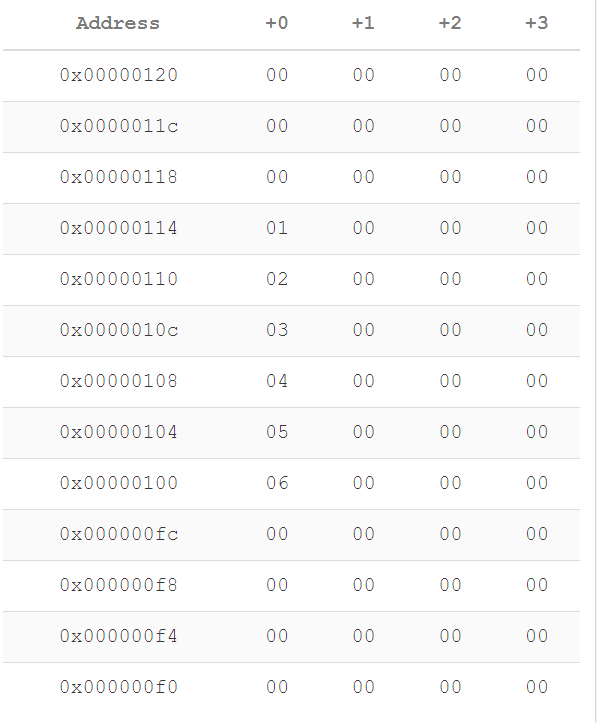
\includegraphics[width=0.8\textwidth]{before.png}
    \caption{Image of Memory before Sorting}
    \label{fig:SelectionSort}
\end{figure}

\begin{figure}[h]
    \centering
    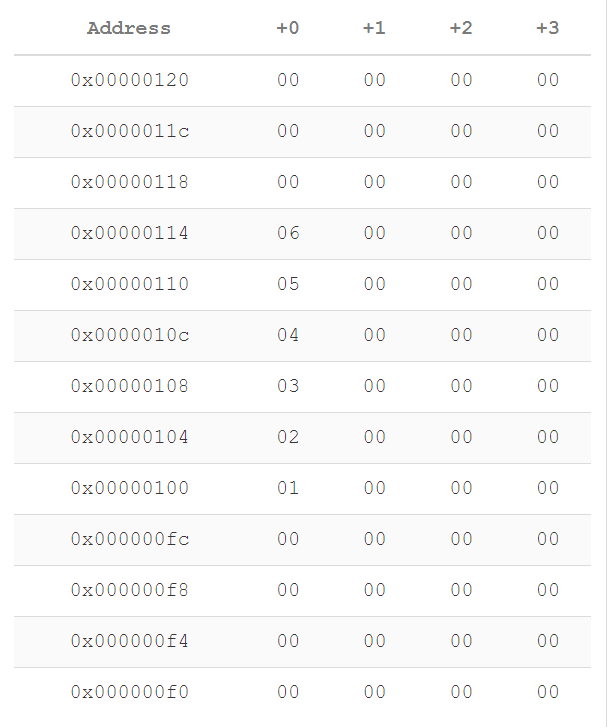
\includegraphics[width=0.8\textwidth]{after.png}
    \caption{Image of Memory after Sorting}
    \label{fig:SelectionSort2}
\end{figure}

% \section{Single Cycle Processor for BLT instruction - Changes}
\newpage

\section{Changes to Single Cycle Processor}

\subsection{Changes to Control Unit}

\begin{lstlisting}[caption={Changes to Control Unit}, captionpos=b, language=RISC-V]
    module Control_Unit
(
	input [6:0] Opcode,
	output reg Branch, MemRead, MemtoReg, MemWrite, ALUSrc, RegWrite,
	output reg [1:0] ALUOp
);

	always @ (Opcode)
	begin
		case (Opcode)
			7`b0110011: //R type (51)
				begin
					Branch = 0;
					MemRead = 0;
					MemtoReg = 0;
					MemWrite = 0;
					ALUSrc = 0;
					RegWrite = 1;
					ALUOp = 2`b10;
				end
			7`b0000011: //ld (3)
				begin
					Branch = 0;
					MemRead = 1;
					MemtoReg = 1;
					MemWrite = 0;
					ALUSrc = 1;
					RegWrite = 1;
					ALUOp = 2`b00;
				end
			7`b0010011: //addi (19)
				begin
					Branch = 0;
					MemRead = 0;
					MemtoReg = 0;
					MemWrite = 0;
					ALUSrc = 1;
					RegWrite = 1;
					ALUOp = 2`b00;
				end

			7`b0100011: // I type SD  (35)
				begin
					Branch = 0;
					MemRead = 0;
					MemtoReg = 1`bx;
					MemWrite = 1;
					ALUSrc = 1;
					RegWrite = 0;
					ALUOp = 2`b00;
				end
			7`b1100011://SB type blt and beq  99
				begin
					Branch = 1;
					MemRead = 0;
					MemtoReg = 1`bx;
					MemWrite = 0;
					ALUSrc = 0;
					RegWrite = 0;
					ALUOp = 2`b01;
				end
			default:
               begin
                ALUSrc   = 1`b0;
                MemtoReg = 1`b0;
                RegWrite = 1`b0;
                MemRead  = 1`b0;
                MemWrite = 1`b0;
                Branch   = 1`b0;
                ALUOp    = 2`b00;     
               end
		endcase				
	end
endmodule
\end{lstlisting}

The input signals to the control unit, which are the OpCode bits 6:0, are used to set the seven control signals. Given that both instructions require jumping to a specific memory address without any reading or writing, the OpCode for beq and blt is the same, as are their signals.
 
\subsection{Changes to ALU Control Unit}

\begin{lstlisting}[caption={Changes to ALU Control Unit}, captionpos=b, language=RISC-V]
module ALU_Control
(
    input [1:0] ALUOp, 
    input [3:0] Funct,
    output reg [3:0] Operation
);

    always @(*)
    begin
        case(ALUOp)
    2`b00:
        begin
        Operation = 4`b0010;
        end
        2`b01:                          // branch type instructions
            begin
            case(Funct[2:0])
            3`b000:                  // beq
                begin
                Operation = 4`b0110;  // subtract
                end
            3`b100:                  // blt
                begin
                Operation = 4`b0100; // less than operation 
                end
                endcase
            end
            
        
        2`b10:
        begin
            case(Funct)
            4`b0000: 
                begin
                Operation = 4`b0010;
                end
                4`b1000:
                begin
                Operation = 4`b0110;
                end
                4`b0111:
                begin
                Operation = 4`b0000;
                end
                4`b0110:
                begin
                Operation = 4`b0001;
                end
            endcase
        end
        endcase
    end    
endmodule
\end{lstlisting}

ALU Control, which creates the 4-bit ALU Control input, has been modified. The Func Field [1-bit from funct7 field (bit 30) plus 3-bits from funct3 field (bits 14:12)] and a 2-bit control field known as ALUOp are inputs to the control unit. The output is a 4-bit signal that, depending on Func and the ALUOp field, selects one of the six operations to be executed in our example, directly controlling the ALU. According to ALUOp, the operation that has to be carried out will either be add (00) for loads and stores or will be determined by the operation that is encoded in the funct7 and funct3 fields (10, 01). When ALUOp was "01," that is, when there was a branch type instruction, we added an additional case structure.

\subsection{Changes to ALU}

\begin{lstlisting}[caption={Changes to ALU 64 bit}, captionpos=b, language=RISC-V]
module ALU_64_bit
    (
        input [63:0]a, b,
        input [3:0] ALUOp,
        
        output reg [63:0] Result,
        output ZERO
    );

    localparam [3:0]
    AND = 4'b0000,
    OR	= 4'b0001,
    ADD	= 4'b0010,
    Sub	= 4'b0110,
    NOR = 4'b1100,
    Less = 4'b0100;

    assign ZERO = (Result == 0);

    always @ (ALUOp, a, b)
    begin
        case (ALUOp)
            AND: Result = a & b;
            OR:	 Result = a | b;
            ADD: Result = a + b;
            Sub: Result = a - b;
            NOR: Result = ~(a | b);
            Less: Result = (a < b) ? 0 : 1;   //less than operation
            
            default: Result = 0;
        endcase
    end

endmodule
\end{lstlisting}

If first value is less than second value, Result is set to `0'. Similar to the beq instruction, `0' would be assigned to Zero if Result $ == $ 0. This eliminates the need for extra hardware modifications to check for additional branch type instructions. In accordance with our hardware structure, where a selection line of mux is Branch \& Zero, the PC is unconditionally replaced with PC + 4 when the Branch control signal is 0, and the branch target is replaced with the PC if the Zero output of the ALU is high (when a b or a b = 0)

% \subsection{Instruction Memory}
% 
% \begin{lstlisting}[caption={Changes to ALU 64 bit}, captionpos=b, language=RISC-V]
% module Instruction_Memory
% (
%     input [63:0] Inst_Address,
%     output reg [31:0] Instruction
% );
%     reg [7:0] inst_mem [147:0];
    
%     initial
%     begin
    
%         //addi x11, x0, 6
%         inst_mem[0]=8'b10010011;
%         inst_mem[1]=8'b00000101;
%         inst_mem[2]=8'b01100000;
%         inst_mem[3]=8'b0;
        
%         //addi x29, x0, 6
%         inst_mem[4]=8'b10010011;
%         inst_mem[5]=8'b00001110;
%         inst_mem[6]=8'b01100000;
%         inst_mem[7]=8'b0;
        
%         //addi x30, x0, 0
%         inst_mem[8]=8'b00010011;
%         inst_mem[9]=8'b00001111;
%         inst_mem[10]=8'b00000000;
%         inst_mem[11]=8'b0;
        
%         //addi x31 x0 0
%         inst_mem[12]=8'b00010011;
%         inst_mem[13]=8'b00001111;
%         inst_mem[14]=8'b00000000;
%         inst_mem[15]=8'b0;
        
%         //addi x28, x0, 6
%         inst_mem[16]=8'b00010011;
%         inst_mem[17]=8'b00001110;
%         inst_mem[18]=8'b01100000;
%         inst_mem[19]=8'b0;
        
%         //sw x11, 256(x30)
%         inst_mem[20]=8'b00100011;
%         inst_mem[21]=8'b00100000;
%         inst_mem[22]=8'b10111111;
%         inst_mem[23]=8'b00010000;
        
%         //addi x31 x31 1
%         inst_mem[24]=8'b10010011;
%         inst_mem[25]=8'b10001111;
%         inst_mem[26]=8'b00011111;
%         inst_mem[27]=8'b0;
        
%         //addi x30 x30 8
%         inst_mem[28]=8'b00010011;
%         inst_mem[29]=8'b00001111;
%         inst_mem[30]=8'b10001111;
%         inst_mem[31]=8'b0;
        
%         //addi x11 x11 -1
%         inst_mem[32]=8'b10010011;
%         inst_mem[33]=8'b10000101;
%         inst_mem[34]=8'b11110101;
%         inst_mem[35]=8'b11111111;
        
%         //beq x28 x31 8
%         inst_mem[36]=8'b01100011;
%         inst_mem[37]=8'b00000100;
%         inst_mem[38]=8'b11111110;
%         inst_mem[39]=8'b00000001;

%         //beq x0 x0 -20
%         inst_mem[40]=8'b11100011;
%         inst_mem[41]=8'b00000110;
%         inst_mem[42]=8'b00000000;
%         inst_mem[43]=8'b11111110;
        
%         //addi x30 x0 0
%         inst_mem[44]=8'b00010011;
%         inst_mem[45]=8'b00001111;
%         inst_mem[46]=8'b00000000;
%         inst_mem[47]=8'b0;
        
%         //addi x31 x30 0
%         inst_mem[48]=8'b10010011;
%         inst_mem[49]=8'b00001111;
%         inst_mem[50]=8'b00001111;
%         inst_mem[51]=8'b0;
        
%         //addi x29 x0 0
%         inst_mem[52]=8'b10010011;
%         inst_mem[53]=8'b00001110;
%         inst_mem[54]=8'b0;
%         inst_mem[55]=8'b0;
        
%         //addi x11 x0 6
%         inst_mem[56]=8'b10010011;
%         inst_mem[57]=8'b00000101;
%         inst_mem[58]=8'b01100000;
%         inst_mem[59]=8'b0;
        
%         //beq x11 x30 88
%         inst_mem[60]=8'b01100011;
%         inst_mem[61]=8'b10001100;
%         inst_mem[62]=8'b11100101;
%         inst_mem[63]=8'b00000101;
        
%         //add x10 x29 x0
%         inst_mem[64]=8'b00110011;
%         inst_mem[65]=8'b10000101;
%         inst_mem[66]=8'b00001110;
%         inst_mem[67]=8'b0;
        
%         //addi x31 x30 1
%         inst_mem[68]=8'b10010011;
%         inst_mem[69]=8'b00001111;
%         inst_mem[70]=8'b00011111;
%         inst_mem[71]=8'b0;
        
%         //addi x28 x29 8
%         inst_mem[72]=8`b00010011;
%         inst_mem[73]=8`b10001110;
%         inst_mem[74]=8`b10001110;
%         inst_mem[75]=8`b0;
        
%         //beq x31 x11 48
%         inst_mem[76]=8`b01100011;
%         inst_mem[77]=8`b10001000;
%         inst_mem[78]=8`b10111111;
%         inst_mem[79]=8`b00000010;
        
%         //lw x15 256(x28)
%         inst_mem[80]=8`b10000011;
%         inst_mem[81]=8`b00100111;
%         inst_mem[82]=8`b00001110;
%         inst_mem[83]=8`b00010000;
        
%         //lw x16 256(x10)
%         inst_mem[84]=8`b00000011;
%         inst_mem[85]=8`b00101000;
%         inst_mem[86]=8`b00000101;
%         inst_mem[87]=8`b00010000;
        
%         //blt x15 x16 28
%         inst_mem[88]=8`b01100011;
%         inst_mem[89]=8`b11001110;
%         inst_mem[90]=8`b00000111;
%         inst_mem[91]=8`b00000001;
        
%         //addi x31 x31 1
%         inst_mem[92]=8`b10010011;
%         inst_mem[93]=8`b10001111;
%         inst_mem[94]=8`b00011111;
%         inst_mem[95]=8`b00000000;
        
%         //addi x28 x28 8
%         inst_mem[96]=8`b00010011;
%         inst_mem[97]=8`b00001110;
%         inst_mem[98]=8`b10001110;
%         inst_mem[99]=8`b00000000;
        
%         //beq x0 x0 -24
%         inst_mem[100]=8`b11100011;
%         inst_mem[101]=8`b00000100;
%         inst_mem[102]=8`b00000000;
%         inst_mem[103]=8`b11111110;
        
%         //addi x30 x30 1
%         inst_mem[104]=8`b00010011;
%         inst_mem[105]=8`b00001111;
%         inst_mem[106]=8`b00011111;
%         inst_mem[107]=8`b0;
        
%         //addi x28 x28 8
%         inst_mem[108]=8`b00010011;
%         inst_mem[109]=8`b00001110;
%         inst_mem[110]=8`b10001110;
%         inst_mem[111]=8`b0;
        
%         //beq x0 x0 -52
%         inst_mem[112]=8`b11100011;
%         inst_mem[113]=8`b00000110;
%         inst_mem[114]=8`b00000000;
%         inst_mem[115]=8`b11111100;
        
%         //addi x10 x28 0
%         inst_mem[116]=8`b00010011;
%         inst_mem[117]=8`b00000101;
%         inst_mem[118]=8`b00001110;
%         inst_mem[119]=8`b0;
        
%         //beq x0 x0 -28
%         inst_mem[120]=8`b11100011;
%         inst_mem[121]=8`b00000010;
%         inst_mem[122]=8`b00000000;
%         inst_mem[123]=8`b11111110;
        
%         //lw x13 256(x10)
%         inst_mem[124]=8`b10000011;
%         inst_mem[125]=8`b00100110;
%         inst_mem[126]=8`b00000101;
%         inst_mem[127]=8`b00010000;
        
%         //lw x14 256(x29)
%         inst_mem[128]=8`b00000011;
%         inst_mem[129]=8`b10100111;
%         inst_mem[130]=8`b00001110;
%         inst_mem[131]=8`b00010000;
        
%         //sw x13 256(x29)
%         inst_mem[132]=8`b00100011;
%         inst_mem[133]=8`b10100000;
%         inst_mem[134]=8`b11011110;
%         inst_mem[135]=8`b00010000;
        
%         //sw x14 256(x10)
%         inst_mem[136]=8`b00100011;
%         inst_mem[137]=8`b00100000;
%         inst_mem[138]=8`b11100101;
%         inst_mem[139]=8`b00010000;
        
%         //addi x29 x29 8
%         inst_mem[140]=8`b10010011;
%         inst_mem[141]=8`b10001110;
%         inst_mem[142]=8`b10001110;
%         inst_mem[143]=8`b0;
        
%         //beq x0 x0 -40
%         inst_mem[144]=8`b11100011;
%         inst_mem[145]=8`b00001100;
%         inst_mem[146]=8`b00000000;
%         inst_mem[147]=8`b11111100;

%     end
    
%     always @(Inst_Address)
%     begin
%         Instruction={inst_mem[Inst_Address+3],inst_mem[Inst_Address+2],inst_mem[Inst_Address+1],inst_mem[Inst_Address]};
%     end
% endmodule
% \end{lstlisting}

% Each instruction of the assembly language selection sort was converted into a 32-bit address.

\subsection{Data Memory}

\begin{lstlisting}[caption={Changes to Data Memory}, captionpos=b, language=RISC-V]
module Data_Memory
(
    input [63:0] Mem_Addr,
    input [63:0] Write_Data,
    input clk, MemWrite, MemRead,
    output reg [63:0] Read_Data
, 
    output [63:0] element1,
    output [63:0] element2,
    output [63:0] element3,
    output [63:0] element4,
    output [63:0] element5,
    output [63:0] element6
);

    reg [7:0] DataMemory [1233:0];

        assign element1 = DataMemory[256];
        assign element2 = DataMemory[264];
        assign element3 = DataMemory[272];                      
        assign element4 = DataMemory[280];
        assign element5 = DataMemory[288];
        assign element6 = DataMemory[296];
        integer i;
    
    initial  
    begin 
        for (i = 0; i < 1233; i = i + 1)
        begin 
        DataMemory[i] = 8`d0;
        end
        end    

    
    always @ (posedge clk)
    begin
        if (MemWrite)
        begin
            DataMemory[Mem_Addr] = Write_Data[7:0];
            DataMemory[Mem_Addr+1] = Write_Data[15:8];
            DataMemory[Mem_Addr+2] = Write_Data[23:16];
            DataMemory[Mem_Addr+3] = Write_Data[31:24];
            DataMemory[Mem_Addr+4] = Write_Data[39:32];
            DataMemory[Mem_Addr+5] = Write_Data[47:40];
            DataMemory[Mem_Addr+6] = Write_Data[55:48];
            DataMemory[Mem_Addr+7] = Write_Data[63:56];
        end
    end
    
    always @ (*)
    begin
        if (MemRead)
            Read_Data = {DataMemory[Mem_Addr+7],DataMemory[Mem_Addr+6],DataMemory[Mem_Addr+5],DataMemory[Mem_Addr+4],DataMemory[Mem_Addr+3],DataMemory[Mem_Addr+2],DataMemory[Mem_Addr+1],DataMemory[Mem_Addr]};
    end
endmodule
\end{lstlisting}

\section{Task 2 - Introducing Pipeline Stages}

A difficulty with implementation of single cycle processor is that the processor only executes one instruction at a time, and only after that instruction is finished is execution of the subsequent instruction begins, which is counter-productive. Given that the majority of the components in our processors would remain idle, it is immediately clear how wasteful this would be and how much processing power it would waste. This is why, in this section, we'll try to fix it by adding pipelining to our single-cycle processor.

Pipelining would allow us to execute numerous commands at once. An in-depth explanation of how this works will be provided in the following section, but for now, consider that one component will work on one portion of the instruction while the other will work on a different part at the same point, thus increasing the efficiency of the whole program. We`ll be incorporating a five-stage pipeline into our Risc-V processor, allowing it to handle five instructions at once. The five stages we implemented for the processor are as follows:

\begin{enumerate}
    \item IF: Instruction Fetch
    \item ID: Instruction Decode 
    \item EX: Execution or address calculation
    \item MEM: Data Memory Access
    \item WB: Write back

\end{enumerate}

We will be introducing four new registers to implement the pipelining stage and to make our program more efficient. These registers are as follows:

\begin{enumerate}
    \item IF/ID register: This register will be used to store the instruction fetched in the IF stage and will be used in the ID stage.
    \item ID/EX register: This register will be used to store the instruction decoded in the ID stage and will be used in the EX stage.
    \item EX/MEM register: This register stores the result of the execution stage.
    \item MEM/WB register: This register stores the result of the memory access stage.
\end{enumerate}

These four newly introduced pipeline registers help in the pipelining process. These registers allow the pipeline to handle multiple instructions simultaneously and keep track of the progress of each instruction as it moves through the pipeline. The use of these registers helps to improve the performance of the processor by enabling the processing of multiple instructions in parallel.

An ideal pipeline would be one which continously moves forward and the instructions are only provided and moved forward. However, this is not the case with the pipeline taught to us. e of the PC, choosing between the
incremented PC and the branch address from the MEM stage. 

Along with the four intermediate pipeline registers, we will also add a control line and a forwarding unit. We extend these registered to store the control lines passed from one stage to another. These registers would be timed to the clock and would either send the stored contents for additional processing or be flushed on each positive edge.

Let us now look at the changes made to the single cycle processor to implement the pipelining. In order to explain the changes made, we will be explaining each pipelining stage separatelty and the significance of the said stage. 

\subsection{Stage 1 - Instruction Fetch (IF)}

Our processor's instruction fetch (IF) step is its initial operation. This stage, as its name implies, is responsible for reading the instruction from memory. To do this, it first determines the address of the instruction to be read through the PC counter, then reads the instruction from the Instruction memory module and sends it to the next stage through the IF/ID register. This also addresses the jump address if it is a problem.

The following is the module used in the stage. 

\begin{lstlisting}[caption={IF/ID Register}, captionpos=b, language=RISC-V]
module IF_ID(
    input clk,
    input reset,
    input [31:0] instruction,
    input [63:0] PC_Out,
    input IF_write,
    output reg [31:0] IF_ID_instruction,
    output reg [63:0] IF_ID_PCOut
    );
    
    always @(posedge clk or reset)
        begin
            if (reset == 1`b1)
                begin
                    IF_ID_instruction = 0;
                    IF_ID_PCOut = 0;
                end
            else if (clk==1 || IF_write == 1)
                begin
                    IF_ID_instruction = instruction;
                    IF_ID_PCOut = PC_Out;
                end
        end   
endmodule
\end{lstlisting}

Before sending everything to the IF/ID register, which on the subsequent clock cycle would transfer the contents to the next step, the following connections are made. The intermediate connections between the Instruction Fetch stage and the Instruction decode stage are made by the outputs from this register.

\subsection{Stage 2 - Instruction Decode (ID)}

Our pipeline's second step is responsible for decoding the instruction, reading from registers, and writing to registers. Therefore, it begins by having the IF stage fetch the instruction. Once the 32-bit instruction has been decoded and its opcode, rd, rs1, and rs2 have been determined, it is then passed on to the instruction parser and the data extractor module. The RegisterFile then reads the contents of the registers or writes back to them (Note that writing back requires signals from the MEM/WEB register, indicating that it is a right-to-left operation, but it doesn't interrupt programme flow).

\begin{lstlisting}[caption={ID/EX Register}, captionpos=b, language=RISC-V]
module ID_EX(
    input clk,
    input reset,
    input branch,
    input MemRead,
    input MemtoReg,
    input MemWrite,
    input ALUsrc,
    input RegWrite,
    input [1:0] ALU_Op, 
    input [63:0] readdata1,
    input [63:0] readdata2,
    input [63:0] immediate,
    input [63:0] pc_out, 
    input [4:0] rs1,
    input [4:0] rs2,
    input [4:0] rd ,
    input[3:0] func,
    output reg branch_out, MemRead_out, MemtoReg_out, MemWrite_out, ALUsrc_out, RegWrite_out, 
    output reg [1:0] AlU_Op_out, 
    output reg [63:0]  readdata1_out,readdata2_out,immediate_out,pc_out_out,
    output reg [4:0] rs1_out, rs2_out, rd_out , 
    output reg [3:0] func_out
    );
    
        always @(*)
        begin
            if (reset==1`b1)
            begin
        
                branch_out = 0; 
                MemRead_out=0;
                MemtoReg_out=0;
                MemWrite_out=0;
                ALUsrc_out=0;
                AlU_Op_out=0;
                RegWrite_out=0;
                readdata1_out=0;
                readdata2_out=0;
                immediate_out=0;
                pc_out_out=0;
                rs1_out= 0;
                rs2_out=0;
                rd_out=0;
                func_out=0;
                
            end 
    else if (clk==1)
    begin     
        MemRead_out=MemRead;
        MemtoReg_out=MemtoReg;
        MemWrite_out=MemWrite;
        ALUsrc_out=ALUsrc;
        AlU_Op_out=ALU_Op;
        RegWrite_out=RegWrite;
        readdata1_out=readdata1;
        readdata2_out=readdata2;
        immediate_out=immediate;
        pc_out_out=pc_out;
        rs1_out= rs1;
        rs2_out=rs2;
        rd_out=rd;
        func_out=func;
        end   
    end 
endmodule

\end{lstlisting}

\subsection{Stage 3 - Execution (EX)}
The third stage of our pipeline is the execution stage. This stage is responsible for performing the following two main tasks. 

\begin{enumerate}
    \item If the instruction is a branch instruction, the adder determines the offset value that must be added in order to determine the address of the subsequent location.
    \item The ALU resides here, so all the operations are executed here.
\end{enumerate}

The value that is to be sent to the registers is controlled by the two MUX after we obtained the ALUop from the Instruction Decode register, which is the control line for the ALU. We now shift our focus as to what exactly is the Execution stage carrying out. 

\begin{lstlisting}[caption={EX/MEM Register}, captionpos=b, language=RISC-V]
module EX_MEM(
    input clk, reset,
    input [4:0] rd,
    input [63:0] write_data , 
    //input branch_MUX,
    input [63:0] ALU_result, PC_out,
    input zero, branch, MemRead, MemWrite, RegWrite, MemtoReg, 
    output reg [4:0] rd_out,
    output reg [63:0] write_data_out, 
    output reg [63:0] ALU_result_out, 
    output reg zero_out, branch_out, MemRead_out, MemWrite_out, RegWrite_out, MemtoReg_out, 
    output reg [63:0] PC_out_out,
    output reg branch_MUX_out
    );

    always @(posedge clk ,posedge reset)
        begin
            if (reset==1)
                begin
                    PC_out_out=0;
                    rd_out = 0;
                    branch_out=0;
                    MemRead_out=0;
                    MemWrite_out=0;
                    RegWrite_out=0;
                    MemtoReg_out=0;
                    write_data_out=0; 
                    ALU_result_out = 0;
                    branch_MUX_out=0;
                    zero_out=0;
                end

        else if (clk==1)
        begin
            PC_out_out=PC_out;
            rd_out=rd ;
            write_data_out=write_data; 
            MemRead_out=MemRead;
            MemWrite_out=MemWrite;
            RegWrite_out= RegWrite ;
            MemtoReg_out=MemtoReg ;
            ALU_result_out=ALU_result ;
            branch_MUX_out=ALU_result ;
            zero_out= zero;
            branch_out=branch;  
        end
    end
endmodule

\end{lstlisting}

\subsection{Stage 4 - Memory Access (MEM)}

The single module at this step is Data Memory, but it also serves as a register for sending back signals, so it checks to see if MemRead or MemWrite is high before carrying out the operation and setting the control lines to write data to or retrieve data from the memory. In order to handle data dangers, this also sends the register contents back to the Execution step for calculations. When the MemWrite signal is high, this register's primary function is to write data to the memory; when the MemRead signal is high, it reads data from the memory into the specified register. As a result, the MEM/WB transmits the register contents as well as additional control signals to the pipeline's final stage. The following stage is implemented into pipelining as follows;

\begin{lstlisting}[caption={MEM/WB Register}, captionpos=b, language=RISC-V]
module MEM_WB(
    input clk,
    input reset,
    input reg_write,
    input memtoreg,
    input [4:0] rd,
    input [63:0] ALU_result,
    input [63:0] read_data,
    output reg reg_write_out,
    output reg mem_to_reg_out,
    output reg [4:0] rd_out,
    output reg [63:0] ALU_result_out,
    output reg [63:0] read_data_out 
    );
       
    always @(posedge clk or reset)
        begin
            if (reset==1`b1)
                begin
                    rd_out = 0;
                    ALU_result_out = 0;
                    read_data_out = 0;
                    reg_write_out= 0;
                    mem_to_reg_out= 0;            	
                end
            else if (clk)
                begin
                    rd_out = rd;
                    ALU_result_out = ALU_result;
                    read_data_out = read_data;
                    reg_write_out= reg_write;
                    mem_to_reg_out= memtoreg;            	
                end
        end        
endmodule
\end{lstlisting}

\section{Task 3 - Circuitry to Detect Hazards}

\subsection{Forwarding Unit}
Let us say we have to run an arbitrary set of instructions on the pipelined version of the processor. 

\begin{lstlisting}[caption={Arbitrary Set of instructions}, captionpos=b, language=RISC-V]
add x1, x2, x3
add x4, x1, x2
\end{lstlisting}

Our processor would now execute the first instruction without issue, but let's try to analyse the second instruction. The second instruction would be in the Instruction decoding stage when the first instruction would be in the execution stage, and as we have seen, this stage is also responsible for reading the values of the register. Therefore, when reading the values stored in the register, the value in x1 for the second instruction should be the sum of the values in x2 and x3. 

We refer to this as a data risk. We have methods like forwarding and stalling to get around this. The latter of the two is the more effective, and that is precisely what we use in our processor. In order to avoid waiting for the value to be loaded into the register before reading from it, forwarding delivers the value immediately after it has been calculated in the execution stage and is required in the ID stage.

A forwarding unit has been implemented in order to take care of hazards such as these. The following is the implementation of a forwarding unit in RISC-V. 

\begin{lstlisting}[caption={Forwarding Unit}, captionpos=b, language=RISC-V]
module Forwarding_Unit(
    input [4:0] ID_EX_Rs1,
    input [4:0] ID_EX_Rs2,
    input [4:0] EX_MEM_Rd,
    input EX_MEM_RegWrite,
    input [4:0] MEM_WB_Rd,
    input MEM_WB_RegWrite,
    output reg [1:0] Forward_A,
    output reg [1:0] Forward_B
    );
    
        always @(*)
            begin
            if (EX_MEM_RegWrite == 1 && EX_MEM_Rd == ID_EX_Rs1 && EX_MEM_Rd != 0)
            begin
                Forward_A = 2`b10;   //10
            end
        else if (MEM_WB_Rd == ID_EX_Rs1 && MEM_WB_RegWrite == 1 && MEM_WB_Rd != 0 &&
                !(EX_MEM_RegWrite == 1 && EX_MEM_Rd != 0 && EX_MEM_Rd == ID_EX_Rs1))
            begin
                Forward_A = 2`b01;  //01
            end
        else

            begin
                Forward_A = 2`b00; //00
            end

        //FORWARD B LOGIC
        if (EX_MEM_RegWrite == 1 && EX_MEM_Rd == ID_EX_Rs2 && EX_MEM_Rd != 0)
            begin
                Forward_B = 2`b10;   //10
            end
        else if (MEM_WB_Rd == ID_EX_Rs2 && MEM_WB_RegWrite == 1 && MEM_WB_Rd != 0 &&
                !(EX_MEM_RegWrite == 1 && EX_MEM_Rd != 0 && EX_MEM_Rd == ID_EX_Rs2))
            begin
                Forward_B = 2`b01;  //01
            end
        else  
            begin
                Forward_B = 2`b00;  //00
            end
        end
endmodule
\end{lstlisting}

Three scenarios should be taken into account for forwarding. The first one is EX Hazard, which sends the output of the preceding instruction to either of the ALU's inputs. The multiplexor will select the value from register EX/MEM if the previous instruction was intended to write to the register file and the write register number was equal to the read register number of ALU inputs A or B. As was noted before, in the event of data hazard, the result is occasionally required directly from the MEM stage since, on occasion, the result is saved many times in a single register. As a result, to obtain the most current one, we take it directly from the MEM stage.

The forwarding logic for forwardA and forwardB is carried out according to the following table of conditions.
\\ \\
\includegraphics*[width = 12.5 cm]{forwardingconditions.png}

\begin{lstlisting}[caption={Four MUX}, captionpos=b, language=RISC-V]
module Four_MUX(
    input [63:0] a, b, c, d, 
    input [1:0] sel, 
    output reg [63:0] mux_result
    );
    
    always @(*)
        begin
          if (sel==2`b00)
            mux_result=a;
          else if (sel ==2`b01)
            mux_result=b;
          else if (sel==2`b10)
            mux_result=c;
          else if (sel==2`b11)
            mux_result=d;    
    end 
endmodule
\end{lstlisting}
    
\subsection{Hazard Detection Unit}
Hazard detection unit is an essential component of pipelined processors that helps to detect and resolve hazards that can occur due to the pipelining of instructions. It enables the processor to handle instruction dependencies and avoid pipeline stalls or data hazards, thereby improving the performance of the processor. The hazard detection unit is implemented in the following way in our processor.

\begin{lstlisting}[caption={Hazard Detection Unit}, captionpos=b, language=RISC-V]
module Hazard_detection_Unit(
    input [4:0] if_id_rs1,
    input [4:0] if_id_rs2,
    input [4:0] id_ex_rd,
    input MemRead,
    output reg muxcontrolbit,
    output reg PC_Write,
    output reg If_id_write
    );
    
    always @(*)    
    begin 
        if ((if_id_rs2==id_ex_rd || if_id_rs1==id_ex_rd) &&  MemRead==1)
        begin
            muxcontrolbit=0;
                PC_Write=0;         
            If_id_write=0;
        end
        
        else 
        begin
            muxcontrolbit=1;
            PC_Write=1;
            If_id_write=1;
        end 
        
    end 
    
endmodule
\end{lstlisting}

The hazard detection unit takes in input signals if\_id\_rs1, if\_id\_rs2, id\_ex\_rd, and MemRead, and outputs three signals muxcontrolbit, PC\_Write, and If\_id\_write.

The inputs if\_id\_rs1 and if\_id\_rs2 represent the two source registers of the instruction that was fetched in the previous cycle. The input id\_ex\_rd represents the destination register of the instruction that was decoded in the previous cycle. The input MemRead is a control signal that indicates whether the current instruction is a load instruction that reads data from memory.

The hazard detection unit checks if any of the source registers of the current instruction match the destination register of the previous instruction, and whether the previous instruction was a load instruction that reads data from memory. If both conditions are true, then there is a data hazard, and the hazard detection unit sets the output signals accordingly. The muxcontrolbit output signal is set to 0, indicating that the multiplexer that selects the input to the register file should choose the result from the MEM/WB pipeline stage instead of the EX/MEM pipeline stage. The PC\_Write and If\_id\_write signals are set to 0, indicating that the current instruction should not update the program counter and the IF/ID pipeline register.

If there is no data hazard, then the hazard detection unit sets the output signals to 1, indicating that the current instruction can proceed without any stall or data forwarding. The muxcontrolbit output signal is set to 1, indicating that the multiplexer should select the result from the EX/MEM pipeline stage. The PC\_Write and If\_id\_write signals are set to 1, indicating that the current instruction should update the program counter and the IF/ID pipeline register.

\begin{lstlisting}[caption={Hazard Detection MUX}, captionpos=b, language=RISC-V]
module Hazard_detection_MUX(
    input sel,
    input branch,
    input MemRead,
    input MemtoReg,
    input MemWrite,
    input ALUsrc,
    input RegWrite,
    input [1:0] ALU_Op,
    output reg branch_eq_hazard,
    output reg MemRead_hazard,
    output reg MemtoReg_hazard,
    output reg MemWrite_hazard,
    output reg ALUsrc_hazard,
    output reg RegWrite_hazard,
    output reg [1:0] ALU_Op_hazard
    );

    always @ (*)
    begin
        if (sel==0)
        begin
            branch_eq_hazard=0;
            MemRead_hazard=0;
            MemtoReg_hazard=0;
            MemWrite_hazard=0;
            ALUsrc_hazard=0;
            RegWrite_hazard=0;
            ALU_Op_hazard=0;
        end 
        if (sel==1)
        begin
            branch_eq_hazard=branch;
            MemRead_hazard=MemRead;
            MemtoReg_hazard=MemtoReg;
            MemWrite_hazard=MemWrite;
            ALUsrc_hazard=ALUsrc;
            RegWrite_hazard=RegWrite;
            ALU_Op_hazard=ALU_Op;
            end 
        
    end 
endmodule
\end{lstlisting}

The multiplexer selects between two sets of input signals based on the value of the sel input. The output signals branch\_eq\_hazard, MemRead\_hazard, MemtoReg\_hazard, MemWrite\_hazard, ALUsrc\_hazard, RegWrite\_hazard, and ALU\_Op\_hazard are set based on the selected input signals.

The input signals to the hazard detection unit are branch, MemRead, MemtoReg, MemWrite, ALUsrc, RegWrite, and ALU\_Op. These signals represent various control signals that determine how an instruction should be executed.

The first set of input signals is selected when the sel input is 0. In this case, all the output signals are set to 0, indicating that there is no hazard. This is the default state of the hazard detection unit.

The second set of input signals is selected when the sel input is 1. In this case, the output signals are set based on the input signals. The branch\_eq\_hazard output signal is set to the value of the branch input, indicating that there is a branch hazard if the branch input is asserted. The MemRead\_hazard output signal is set to the value of the MemRead input, indicating that there is a memory read hazard if the MemRead input is asserted. The MemtoReg\_hazard output signal is set to the value of the MemtoReg input, indicating that there is a memory-to-register hazard if the MemtoReg input is asserted. The MemWrite\_hazard output signal is set to the value of the MemWrite input, indicating that there is a memory write hazard if the MemWrite input is asserted. The ALUsrc\_hazard output signal is set to the value of the ALUsrc input, indicating that there is an ALU source hazard if the ALUsrc input is asserted. The RegWrite\_hazard output signal is set to the value of the RegWrite input, indicating that there is a register write hazard if the RegWrite input is asserted. The ALU\_Op\_hazard output signal is set to the value of the ALU\_Op input, indicating that there is an ALU operation hazard if the ALU\_Op input is asserted.

\section{Results}
We will now test our final design. We will check if the pipelined processor is working as intended. 

\begin{figure}[h]
    \centering
    \includegraphics*[width = 13 cm]{loadingvalues.jpeg}
    \caption{Loading the set of inputs}
    \label{fig: label 1}
\end{figure}

Firstly, checking if the values are being loaded into the processor correctly. 

\begin{figure}[h]
    \centering
    \includegraphics*[width = 13 cm]{firstsorting.jpeg}
    \caption{Sorting the set of inputs}
    \label{fig: label 2}
\end{figure}

Checking if the sorting is working correctly and the following is our final sorted result. 

\begin{figure}[h]
    \centering
    \includegraphics*[width = 13 cm]{final_sorted.jpeg}
    \caption{Final Sorted set of elements}
    \label{fig: label 3}
\end{figure}

\newpage

The final thing is to check if the forwarding is working correctly according to the conditions put in place for the forwarding unit to work correctly.

\begin{figure}[h]
    \centering
    \includegraphics*[width = 13 cm]{forwarding.jpeg}
    \caption{Result of Forwarding Unit}
    \label{fig: label 4}
\end{figure}

\subsection{Comparison between Pipelined and non-Pipelined Single Cycle Processor}

Performance for a pipelined Single-cycle processor will be better when compared to a non-pipelined single cycle processor. A pipelined processor and a non-pipelined processor are both single processors, but they differ in how they handle instructions.

A non-pipelined processor executes each instruction in a sequential manner, meaning it completes one instruction before moving on to the next. This can lead to inefficiencies because there may be unused portions of the processor during the execution of an instruction. On the other hand, a pipelined processor breaks down the execution of each instruction into several stages and allows multiple instructions to be processed at the same time. As a result, there is no idle time for the processor, and instructions are executed more quickly.

A pipelined processor is generally faster and more efficient than a non-pipelined processor because it can process instructions simultaneously and this is exactly what we have seen over the course of this semester and the project. However, while designing a pipelined single-cycle processor, one has to keep in mind to not add bottlenecks and add remedies to data hazards for the processor to work efficiently.

\section{Final Comments}
The project has been a unique challenge in a way that it required tedious amounts of debugging the code and modules to figure out what the problem is. At times even after hours of trying to figure out the problem, we could not reach to a correct conclusion. As a result, branching has not been implemented properly in our project, while forwarding unit and hazard detection is working. The failure to implement branching correctly is not down to a lack of effort and time, but guessing it is rather down to a very small error which is not visible to the eye. 


\section{Github Repository}

\href{https://github.com/HammadxSaj/CA-Project}{https://github.com/HammadxSaj/CA-Project}
\end{document}
 